\begin{table}
\begin{center}
\begin{tabular}{|c|p{1cm}|p{1cm}|p{1cm}|}
\hline
Faulty Service & $L_1$ (30ms) & $L_2$ (35ms) & $L_3$ (45ms) \\ \hline
datastore & 18 & 11 & 10 \\ \hline
user management & 19 & 15 & 10 \\ \hline
\end{tabular}
\end{center}
\caption{Number of anomalies detected in guestbook app under different SLOs 
($L_1$, $L_2$ and $L_3$) when injecting faults into two different PaaS kernel services.
\label{tab:anomaly_counts}
}
\end{table}

We first evaluate the effectiveness of Roots as an anomaly detection mechanism. We experiment with
the SLO-based anomaly detector, using a simple HTML-producing web application called ``guestbook''.
This application allows users to login, and post comments. It uses the datastore service to save
the posted comments, and the user management service to handle authentication. We conduct all
of our experiments on a single node AppScale cloud except where specified. The node itself is an Ubuntu
14.04 VM with 4 virtual CPU cores (clocked at 2.4GHz) and 4GB of memory.

We run the SLO-based anomaly detector on guestbook with a sampling rate of 15 seconds, an analysis
rate of 60 seconds, and a window size of 1 hour. We set the minimum sample count to 100, and
run a series of experiments with different SLOs on the guestbook application. Specifically, we fix
the SLO probability at 95\%, and set the response time upper bound to $\mu_g + n\sigma_g$. 
$\mu_g$ and $\sigma_g$ represent mean and standard deviation of the
guestbook's response time. We learn these two parameters apriory by benchmarking
the application. Then we obtain three different upper bound values for the guestbook's
response time by setting 
$n$ to 2, 3 and 5. We denote the resulting three SLOs $L_1$, $L_2$ and $L_3$ respectively.

We also inject performance faults into AppScale by modifying its code. We run a set of experiments
by injecting faults into the datastore service. Our fault injection logic activates once every hour, and
slows down all datastore invocations by 45ms within a period of 3 minutes. 45ms is equal 
to $\mu_g + 5\sigma_g$. Therefore this delay is sufficient to violate all three SLOs used in our experiments. 
We run a similar set of experiments where we inject faults into the user management service of
AppScale. Each experiment is run for a period of 10 hours.

Table~\ref{tab:anomaly_counts} shows how the number of anomalies detected by 
Roots in a 10 hour period varies when the SLO is changed. The number of anomalies
drops noticeably when the response time upper bound is increased. When the $L_3$
SLO (45ms) is used, the only anomalies detected are the ones
caused by our hourly fault injection mechanism. As the SLO is tightened by lowering the upper bound,
Roots detects additional anomalies. These additional anomalies
result from a combination of injected faults, and other naturally occurring faults
in the system.

Next we analyze how fast and often Roots can detect anomalies in an application. We
first consider the performance of guestbook under the $L_1$ SLO while 
injecting faults into the datastore service. Figure~\ref{fig:time_line_guestbook_2s} shows
anomalies detected by Roots as events on a time line. The horizontal axis represents 
passage of time. The red markers indicate the time windows in which we injected faults into
AppScale. Each window is 3 minutes wide, and therefore appears thin in the full 10 hour scale
of the plot. The tall blue lines indicate the Roots anomaly detection events.
Note that every fault injection window is immediately followed by an anomaly
detection event, implying near real time reaction from Roots. The only exception is the fault
injection window at 20:00 hours which is not immediately followed by an anomaly 
detection event. Roots detected another naturally occurring anomaly at 19:52 hours
which caused the anomaly detector to go into the warm up mode. Therefore Roots
did not immediately react to the faults injected at 20:00 hours. But as soon as the detector became
active again at 20:17, it detected the anomaly.

\begin{figure}
\centering
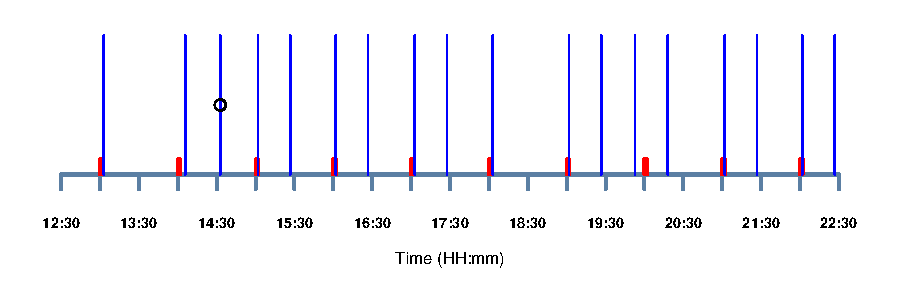
\includegraphics[scale=0.55]{time_line_guestbook_2s}
\caption{Anomaly detection in guestbook application (timeline).}
\label{fig:time_line_guestbook_2s}
\end{figure}

\begin{figure}
\centering
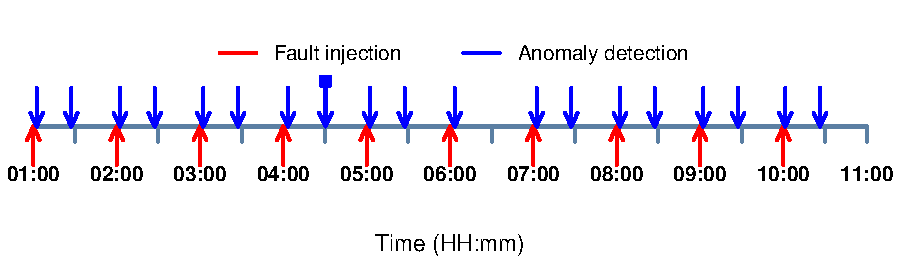
\includegraphics[scale=0.55]{time_line_guestbook_2s_user}
\caption{Anomaly detection in guestbook application (timeline).}
\label{fig:time_line_guestbook_2s_user}
\end{figure}

Figure~\ref{fig:time_line_guestbook_2s_user} shows the anomaly detection time line for the 
same application and SLO, while faults are being injected into the user management service.
Here too we see that Roots detects anomalies immediately following each fault injection window.

\begin{figure}
\centering
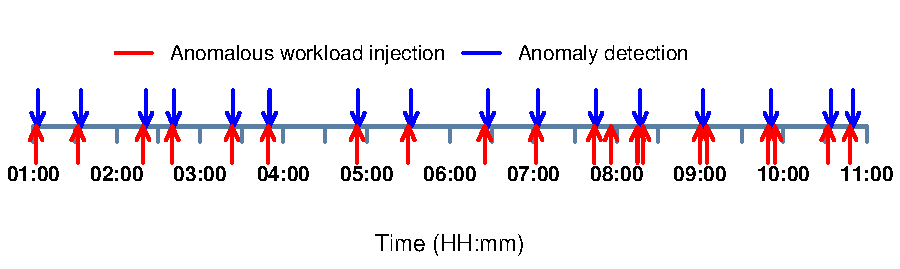
\includegraphics[scale=0.55]{time_line_crud}
\caption{Anomaly detection in key-value store application (timeline).}
\label{fig:time_line_crud}
\end{figure}

\begin{figure}
\centering
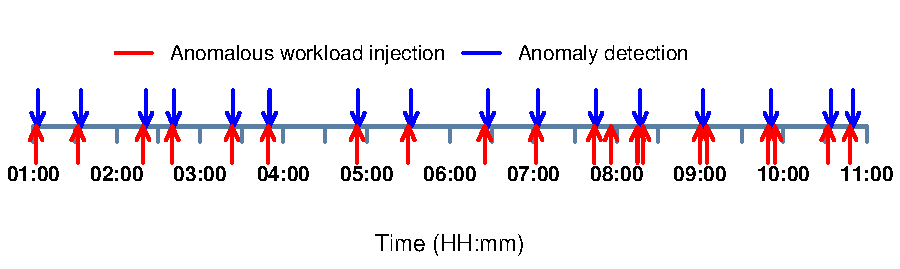
\includegraphics[scale=0.55]{time_line_caching}
\caption{Anomaly detection in caching application (timeline).}
\label{fig:time_line_caching}
\end{figure}

Next we evaluate the effectiveness and accuracy of the path distribution analyzer. For this we 
employ two applications.
\begin{description}
\item[key-value store] Provides the functionality of an online key-value store.  It allows 
users to store data objects in the cloud where each object is given a unique key. The objects can then be 
retrieved, updated or deleted using their keys. Different operations
(create, retrieve, update and delete) of the application are implemented as separate paths of
execution in the application source code.
\item[cached key-value store] A simple extension of the regular key-value store, which adds
caching to the read operation using the AppScale's memcache service. The application contains
separate paths of execution for cache hits and cache misses.
\end{description}

We first deploy the key-value store on AppScale, and populate it with a number of data objects. Then we
run a test client against it which generates a mostly-read workload. On average this workload
consists of 90\% read requests and 10\% write requests (create and update). The test client
is also programmed to randomly send bursts of mostly-write workloads. These bursts consist
of 90\% write requests on average, and each burst lasts up to 2 minutes.

Then we deploy the cached key-value store on AppScale, and run a test client that generates a workload
that is mostly served from the cache. This is done by repeatedly executing read requests on a small
selected set of object keys. However, the client randomly sends bursts of traffic requesting keys that
are not likely to be in the application cache, thus resulting in many cache misses. Each burst
lasts up to 2 minutes. As shown in 
figure~\ref{fig:time_line_caching}, Roots path distribution analyzer correctly detects the change 
in the workload (from many cache hits to many cache misses), every time the test client injects a 
burst of traffic that triggers the cache miss path of the application to get executed.

\begin{figure}
\centering
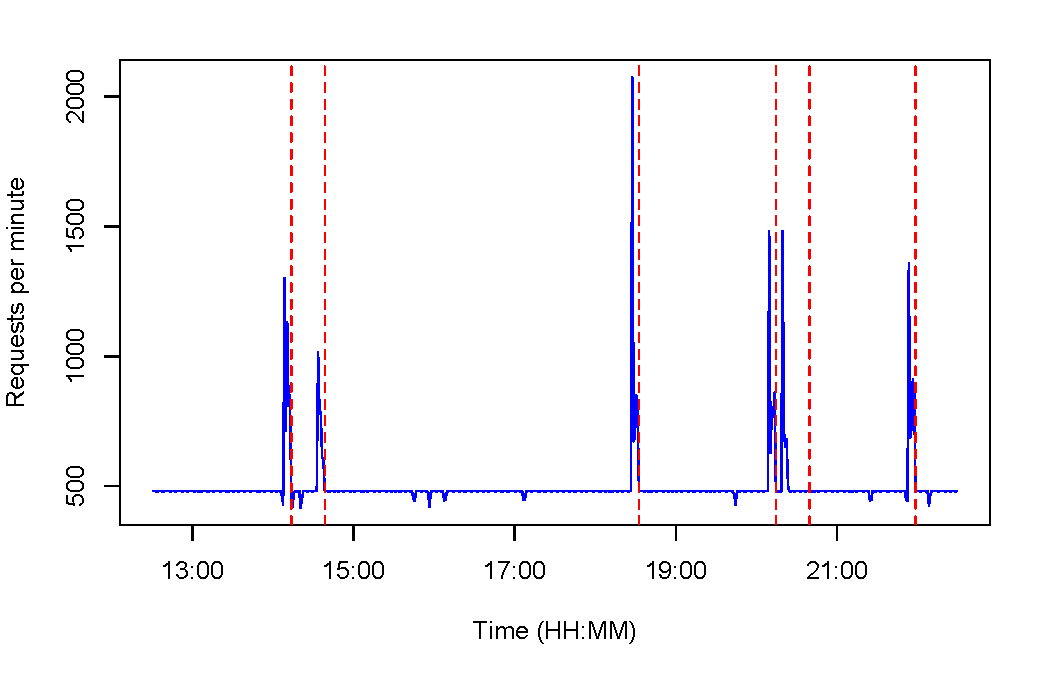
\includegraphics[scale=0.5]{workload_change_trace}
\caption{Workload size over time for the guestbook application. The test client randomly sends
large bursts of traffic causing the spikes in the plot. Roots anomaly detection events are shown
in red dashed lines.}
\label{fig:workload_change}
\end{figure}

Next we evaluate the Roots workload change analyzer. In this experiment we run a varying workload
against the guestbook application for 10 hours. The load generating client is programmed
to maintain a mean workload level of 500 requests per minute. However, the client
is also programmed to randomly send large bursts of traffic at times of its choosing. During these bursts 
the client may send more than 1000 requests a minute, thus impacting the performance of
the application server that hosts the guestbook application. Figure~\ref{fig:workload_change} shows how
the application workload has changed over time. The workload generator has produced 6 large bursts of traffic during the 
period of the experiment, which appear as tall spikes in the plot.
Note that each burst is immediately followed by a Roots anomaly detection event (shown by red dashed lines). 
In each of these 6 cases, the increase in workload caused a violation of the application performance SLO.
Roots detected the corresponding anomalies, and determined them to be caused by changes in the workload size.
Even though the bursts of traffic appear to be momentary
spikes, each burst lasts for 4 to 5 minutes thereby causing a lasting impact on the application performance.
The PELT change point detection method used in this experimental set up is ideally suited for detecting
such lasting changes in the workload level.
